\documentclass{article}

\usepackage{fancyhdr}
\usepackage{extramarks}
\usepackage{amsmath}
\usepackage{amsthm}
\usepackage{amsfonts}
\usepackage{tikz}
\usepackage[plain]{algorithm}
\usepackage{algpseudocode}
\usepackage{hyperref}
\usepackage{caption}
\usepackage{subcaption}
\usepackage{minted}
\usepackage{pdflscape}
\usepackage{listings}
\usepackage{color}

\usetikzlibrary{automata,positioning}

%
% Basic Document Settings
%

% Custom sectioning
\usepackage{sectsty}
\allsectionsfont{\centering \normalfont\scshape}

\captionsetup{justification=centering,
singlelinecheck=false
}
\graphicspath{ {required/} }

\topmargin=-0.45in
\evensidemargin=0in
\oddsidemargin=0in
\textwidth=6.5in
\textheight=9.0in
\headsep=0.25in

\linespread{1.1}

\pagestyle{fancy}
\lhead{\hmwkAuthorName}
\chead{\hmwkClass}
\rhead{\hmwkTitle}
\lfoot{\lastxmark}
\cfoot{\thepage}

\renewcommand\headrulewidth{0.4pt}
\renewcommand\footrulewidth{0.4pt}

\setlength\parindent{0pt}

%
% Create Problem Sections
%

\newcommand{\enterProblemHeader}[1]{
    \nobreak\extramarks{}{Problem \arabic{#1} continued on next page\ldots}\nobreak{}
    \nobreak\extramarks{Problem \arabic{#1} (continued)}{Problem \arabic{#1} continued on next page\ldots}\nobreak{}
}

\newcommand{\exitProblemHeader}[1]{
    \nobreak\extramarks{Problem \arabic{#1} (continued)}{Problem \arabic{#1} continued on next page\ldots}\nobreak{}
    \stepcounter{#1}
    \nobreak\extramarks{Problem \arabic{#1}}{}\nobreak{}
}

\setcounter{secnumdepth}{0}
\newcounter{partCounter}
\newcounter{homeworkProblemCounter}
\setcounter{homeworkProblemCounter}{1}
\nobreak\extramarks{Problem \arabic{homeworkProblemCounter}}{}\nobreak{}

%
% Homework Problem Environment
%
% This environment takes an optional argument. When given, it will adjust the
% problem counter. This is useful for when the problems given for your
% assignment aren't sequential. See the last 3 problems of this template for an
% example.
%
\newenvironment{homeworkProblem}[1][-1]{
    \ifnum#1>0
        \setcounter{homeworkProblemCounter}{#1}
    \fi
    \section{Problem \arabic{homeworkProblemCounter}}
    \setcounter{partCounter}{1}
    \enterProblemHeader{homeworkProblemCounter}
}{
    \exitProblemHeader{homeworkProblemCounter}
}

%
% Homework Details
%   - Title
%   - Due date
%   - Class
%   - Section/Time
%   - Instructor
%   - Author
%

\newcommand{\hmwkTitle}{Homework\ 2}
\newcommand{\hmwkDueDate}{January 30, 2015}
\newcommand{\hmwkClass}{Information Integration on the Web}
\newcommand{\hmwkClassInstructor}{Prof. Ambite \& Knoblock}
\newcommand{\hmwkAuthorName}{Tushar Tiwari}

%
% Title Page
%

\title{
    \vspace{2in}
    \textmd{\textbf{\hmwkClass:\ \hmwkTitle}}\\
    \normalsize\vspace{0.1in}\small{Due\ on\ \hmwkDueDate}\\
    \vspace{0.1in}\large{\textit{\hmwkClassInstructor}}
    \vspace{3in}
}

\author{\textbf{\hmwkAuthorName}}
\date{}

\renewcommand{\part}[1]{\textbf{\large Part \Alph{partCounter}}\stepcounter{partCounter}\\}

%
% Various Helper Commands
%

% Useful for algorithms
\newcommand{\alg}[1]{\textsc{\bfseries \footnotesize #1}}

% For derivatives
\newcommand{\deriv}[1]{\frac{\mathrm{d}}{\mathrm{d}x} (#1)}

% For partial derivatives
\newcommand{\pderiv}[2]{\frac{\partial}{\partial #1} (#2)}

% Integral dx
\newcommand{\dx}{\mathrm{d}x}

% Alias for the Solution section header
\newcommand{\solution}{\textbf{\large Solution}}

% Probability commands: Expectation, Variance, Covariance, Bias
\newcommand{\E}{\mathrm{E}}
\newcommand{\Var}{\mathrm{Var}}
\newcommand{\Cov}{\mathrm{Cov}}
\newcommand{\Bias}{\mathrm{Bias}}
\begin{document}

\maketitle

\pagebreak

\begin{flushleft}
\section{Json of chosen artwork}
\urldef\myurl\url{http://collections.lacma.org/node/184481}
\begin{figure}[H]
\centering
\inputminted[frame=single,
               framesep=3mm,
               linenos=true,
               xleftmargin=21pt,
               tabsize=4]{js} {required/output.json}
\caption{The painting can be found at \myurl.}
\end{figure}

\newpage
\section{RDF Graph}
\begin{figure}[H]
\centering
\fbox{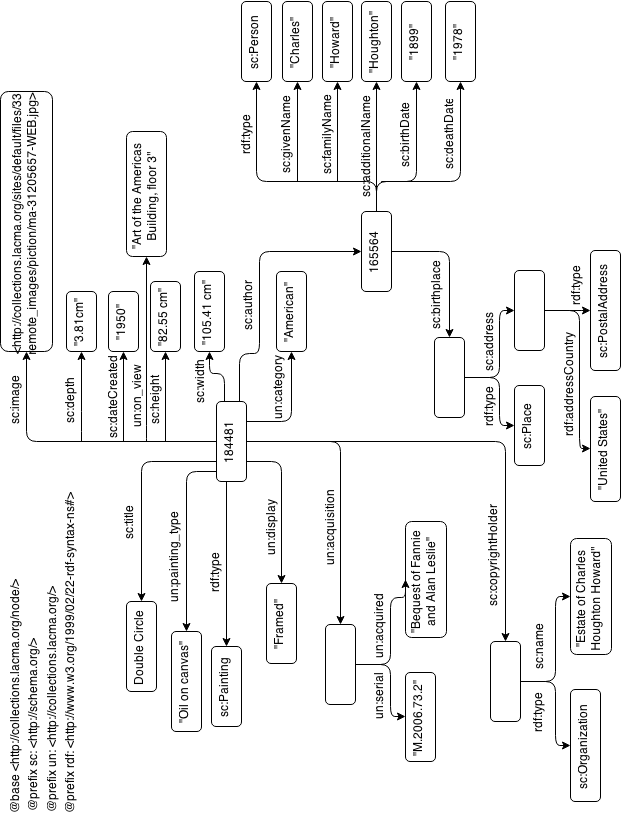
\includegraphics[width=0.98\textwidth]{painting-rotated}}
\caption{The RDF Graph for the above JSON}
\end{figure}

\newpage
% Language Definitions for Turtle
\definecolor{olivegreen}{rgb}{0.2,0.8,0.5}
\definecolor{grey}{rgb}{0.5,0.5,0.5}
\lstdefinelanguage{ttl}{
sensitive=true,
morecomment=[l][\color{grey}]{@},
morecomment=[l][\color{olivegreen}]{\#},
morestring=[b][\color{blue}]\",
showstringspaces=false,
}
\lstset{%
  numbers=none,
  tabsize=4,
  breaklines=true,
  basicstyle=\small\ttfamily,
  framerule=10pt,
  columns=fullflexible,
  language=ttl
}
\section{Turtle triples}
\lstinputlisting{required/query.ttl}

\newpage
\section{Any23.org Report}
\begin{figure}[H]
\centering
\fbox{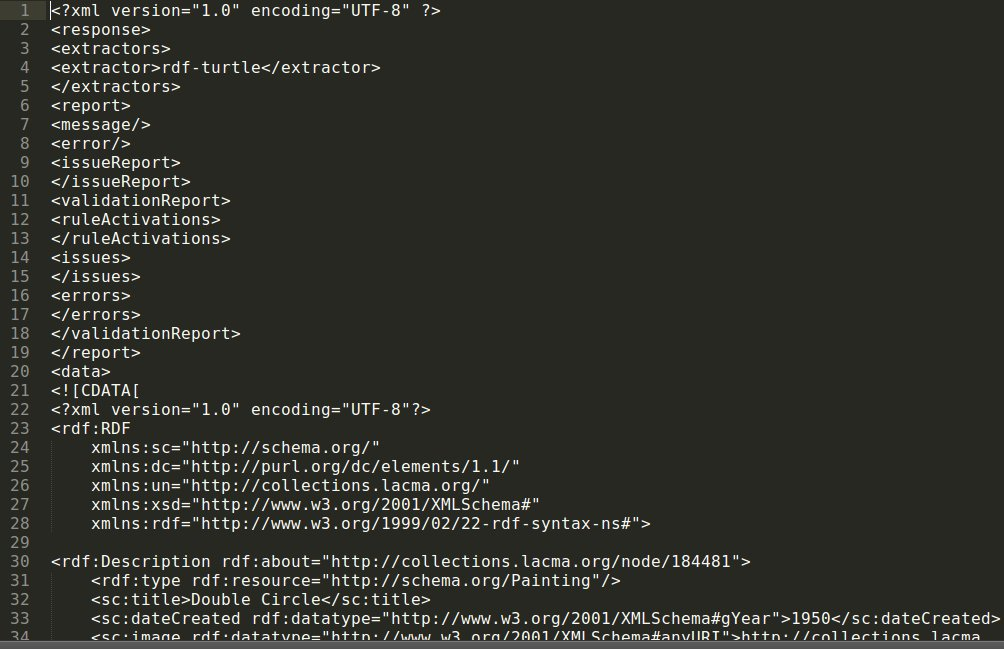
\includegraphics[width=0.98\textwidth]{validated}}
\caption{The empty issues tag under the validationReport tag indicates\\that the turtle code had no errors.}
\end{figure}

\end{flushleft}
\end{document}